\chapter{Evaluation}
In this chapter, the developed components are evaluated through specific individual tests.
These tests do not only cover the actual components making up the Printing Stack, but also verify the correctness of the Skip List implementation.


\section{Verifying The Random Number Generator}
In Section~\ref{sec:FastRNG}, a fast Random Number Generator has been developed that is designed to return geometrically distributed numbers denoting Skip List levels.
The probability parameter of this Generator is defined as $p = 0.5$.
Achieving a sufficiently geometric distribution of Skip List levels is crucial for the Skip List performance.
The average complexity of the algorithms involved cannot be reached if the Skip List levels follow a different distribution.

To verify the distribution of levels returned by the Random Number Generator, a test application has been written.
It calls the Random Number Generator a predefined number of times to simulate the distribution of levels for a Skip List with the same element count.
Logarithmic plots of the results of simulations with 1000 and 65536 elements are provided in Figure~\ref{fig:ElementDistribution}.

In both cases, the results show an approximate geometric distribution for the lower levels with some outliers for higher levels.
As the number of elements is significantly lower on higher levels, these outliers are negligible.
Generally spoken, the more elements are added to a Skip List, the more their assigned levels converge to a geometric distribution.
In total, this test shows that the implemented Random Number Generator is feasible to get the desired distribution for the Skip List algorithms.

\begin{figure}[t]
	\centering
	
	\begin{tikzpicture}
		\begin{axis}[
			scale=0.75,
			title={1000 Elements},
			xlabel={Level},
			xmax=16,
			ymin=0.5,
			ylabel={Element Count},
			ymode=log,
			log basis y=2,
			ytick={1,8,64,512}
		]
			\addplot table {plots/16_levels_1000_elements.csv};
		\end{axis}
	\end{tikzpicture}
	\hspace{8mm}
	\begin{tikzpicture}
		\begin{axis}[
			scale=0.75,
			title={65536 Elements},
			xlabel={Level},
			xmax=16,
			ymin=0.5,
			ymode=log,
			log basis y=2,
			ytick={1,32,1024,32768}
		]
			\addplot table {plots/16_levels_65536_elements.csv};
		\end{axis}
	\end{tikzpicture}
	
	\caption{Distribution of 1000 and 65536 elements across the levels of a 16-level Skip List using the Minimal Standard Random Number Generator}
	\label{fig:ElementDistribution}
\end{figure}


\section{Testing The Skip List Implementation}
As the Skip List is an integral component of the developed Printing Stack, its algorithms received additional unit testing.
In particular, the Skip List for the Printing Stack includes distance arrays for each element to allow a fast lookup of element indexes.
This requires the insertion and deletion functions to update both pointers and distances with every operation.

To test all implemented Skip List functions, another test program has been written.
It utilizes a Skip List that manages plain integer numbers and sorts them in ascending order.
The test first adds 40 random numbers to the list.
In a next step, all numbers in the range 0 to 29 are deleted again.
Finally, another batch of 40 random numbers is added to the Skip List.
Two lookup operations are performed afterwards, one by index and one by looking for a specific integer.
In the end, the structure of the final Skip List is drawn on the screen.
The drawing process makes use of both the pointer and distance information.
An exemplary output of the test program is depicted in Figure~\ref{fig:skiplist_test}.

By calling these individual functions in this specific order, all aspects of the Skip List are tested.
Typical bugs in abstract data type implementations can be caught, like corrupted structures after an operation, off-by-one mistakes in loops, or similar.
The final dump of the resulting structure allows a visual check of the entire Skip List.
In case of a bad link to a next element or a wrongly calculated distance, an element would appear misaligned.

\begin{figure}[b]
	\centering
	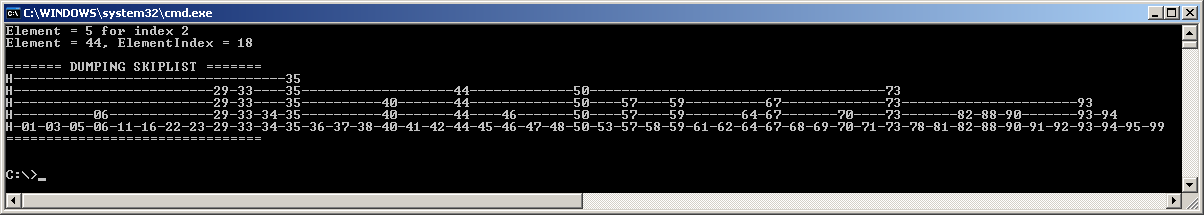
\includegraphics{images/skiplist_test.png}
	\caption{Exemplary output of the Skip List test program}
	\label{fig:skiplist_test}
\end{figure}


\section{Testing The ReactOS Printing Stack In A Virtual Machine}
After individual tests of crucial components, the developed Printing Stack as a whole needed to be tested.
This has been accomplished by building an ISO~9660 image file for the entire ReactOS Operating System, including the newly developed Printing Stack components and the \emph{winspool\_print} test program.
The ReactOS Build System provides the target \emph{bootcd} for this purpose.
Calling this CMake target builds all operating system components and finally creates an ISO~9660 image file.
Instead of using the default GCC compiler, the operating system has been built using Microsoft Visual C++.
This creates the necessary \gls{PDB} files to enable source-level debugging with WinDbg.

As neither Printer Drivers nor Printer Setup functions exist at this stage of the Printing Stack, Printers cannot be installed through the operating system yet.
Without an installed Printer, the Printing Stack cannot be tested though.
To circumvent this problem, the ReactOS installation data has been modified to always set up a dummy Printer connected to the first Parallel Port.
Without a corresponding Printer Driver, this dummy Printer is still able to forward RAW data to the connected real Printer.
As no other datatype nor datatype conversions are supported by now, such a dummy Printer is sufficient for all testing scenarios.

To catch outstanding code bugs early, it has been decided to use a Virtual Machine for testing.
This allows to develop and test on the same computer as well as mounting the created ISO~9660 image file in a virtual CD drive instead of burning it to a blank CD.
While many different Virtualization products exist today, only some were suitable for evaluating the Printing Stack.
This is due to the fact that the Printing Stack outputs data over a Parallel Port.
For this purpose, the free \href{http://www.vmware.com/products/player}{VMware Player} software turned out to be a viable solution, because it offers a virtual Parallel Port, whose output can be redirected into a file.
The returned data can then be examined to validate the correctness of the Printing Stack.

VMware Player has also been configured to emulate a virtual Serial Port and redirect this one to a bidirectional pipe.
The WinDbg debugger can then connect to this pipe and act like it was debugging ReactOS on a computer connected through a physical Serial Cable.

By the use of VMware and WinDbg, several bugs have been caught and fixed in a relatively short time.
Using a Virtual Machine instead of Real Hardware for these tests has also simplified the deployment of fixes:
System components could be exchanged by turning off the Virtual Machine, mounting its virtual Hard Disk on the Host Computer and rebooting ReactOS.

At the end of the testing and fixing phase, the Printing components have finally become robust enough for the \emph{winspool\_print} tool.
The set of implemented \gls{API} calls can be used reliably to send RAW Printing data to the Parallel Port.
Examination of the redirected Parallel Port output has revealed that a Printer would receive properly formatted data.


\section{Running The ReactOS Printing Stack On Real Hardware}
The final evaluation of the developed Printing Stack happened on a real computer connected to a physical Printer.
For this test, a Lenovo ThinkPad X61 with Docking Station has been chosen.
This machine's hardware components are known to be supported by ReactOS out of the box without relying on third-party hardware drivers.
The Docking Station offers Parallel and Serial Ports not provided by the laptop itself.

Preferably, a Dot-Matrix Printer would have been connected to the Parallel Port of this laptop.
Such Printers work character-wise, meaning that they do not await a full page in a Control Language, but output every transmitted character as soon as it arrives.
Due to the unavailability of a Dot-Matrix Printer at the time of testing, a Hewlett-Packard DeskJet 710C Inkjet Printer has been chosen instead.
This particular Printer expects all incoming data in Hewlett-Packard's proprietary \gls{PPA} Control Language.
The \gls{PPA} Language is implemented into the included Windows Device Driver, but otherwise largely undocumented.
However, Windows Printer Drivers are not usable in ReactOS before the \gls{GDI} part of the Printing Stack has been implemented.
Therefore, another solution was necessary to prepare data in \gls{PPA} Language.

This solution has been found in the \emph{PNM2PPA} tool.
PNM2PPA is a program that converts an input image in Portable Pixmap raster format into appropriate \gls{PPA} data for supported Hewlett-Packard Printers \cite{pnm2ppa2015}.
It is usually used in conjunction with the GhostScript software, which converts documents in PostScript language into raster formats.
Together both applications build a filter chain for \gls{CUPS} users to let them print on \gls{PPA} Printers.

As a result of this, a single page document was prepared on a different computer.
This document was first converted into PostScript, then processed into a raster image using GhostScript until PNM2PPA finally produced data in \gls{PPA} format.
The created \gls{PPA} file was then transferred to the laptop running ReactOS.
Finally, the \emph{winspool\_print} tool read the \gls{PPA} file and transmitted correctly formatted data to the DeskJet Printer using \gls{API} functions of the Printing Stack.
The Printer reacted accordingly and printed out the previuosly prepared document.

This final step of testing has shown that the implemented features of the Printing Stack can properly communicate with Printers.
